\chapter[Introduction aux microarchitectures]{Introduction aux microarchitectures \it{Contrôleur-Datapath}}
\minitoc

\section{Introduction}
\lettrine{L} es chapitres précédents nous ont permis de nous doter de circuits de bases : circuits pour l'arithmétique et automates.
Le présent chapitre présente l'assemblage typique de ces deux classes de circuits. Cet assemblage va nous permettre de monter en complexité,
et nous rapprocher progressivement de vrais calculateurs "utiles". Cet assemblage correspond à un "pattern" ou "motif de conception" très répandu, utilisé par
un grand nombre de concepteurs. Ce pattern est une recette de cuisine, qui a été suffisamment éprouvée, pour retenir l'adhésion. Il est par ailleurs
la cible d'outils de synthèse avancés, qui permettent de générer automatiquement des architectures matérielles, à partir de code logiciel.
Mais ceci est une autre histoire (synthèse de haut niveau ou comportementale), qui sera traitée en seconde année...

\section{Chemin de données : architecture générique}
Le schéma \ref{fig:fsmd1} suivant présente un chemin de données (ou datapath) typique : c'est un assemblage de port d'entrées et de sorties, de registres, de multiplexeurs et d'opérateurs de calcul.
Parmi les opérateurs de calcul, on est à même d'y voir :
\begin{itemize}
  \item des opérateurs arithmétiques : additionneurs, multiplieurs, etc
  \item des opérateurs logiques : and, or etc sur des vecteurs de bits
  \item des opérateurs de comparaison : plus-grand-que, test d'égalité etc
  \item ces opérateurs sont généralement regroupés au sein d'une {\it Unité Arithmétique et Logique} (UAL ou ALU en anglais), représentée en jaune sur la figure.
\end{itemize}

Le motif générique permet de comprendre comment on cherche à utiliser ces opérateurs :
\begin{itemize}
  \item les entrées sont acheminées dans un registre.
  \item les opérandes des opérateurs sont multiplexés, c'est-à-dire peuvent provenir de différents registres.
  \item on peut indiquer à une ALU quelle opération elle est censée réaliser.
  \item le résultat d'un opérateur est lui-même soit stocké dans un registre.
\end{itemize}

Dans tous les cas, les {\bf multiplexeurs} y joue un rôle fondamental : les commandes des multiplexeurs permettent d'effectuer des choix entre plusieurs sources.
On observera par ailleurs le caractère synchrone du datapath : le cycle d'horloge permet de réaliser sélectionner les sources nécessaire au calcul, de les router,
de réalser effectivement le calcul et de stocker le résultat. Le cycle d'horloge comment aux registres (précisement aux sorties Q des bascules) et se termine aux entrées
des mêmes registres.

\begin{figure}[h!]
  \centering
   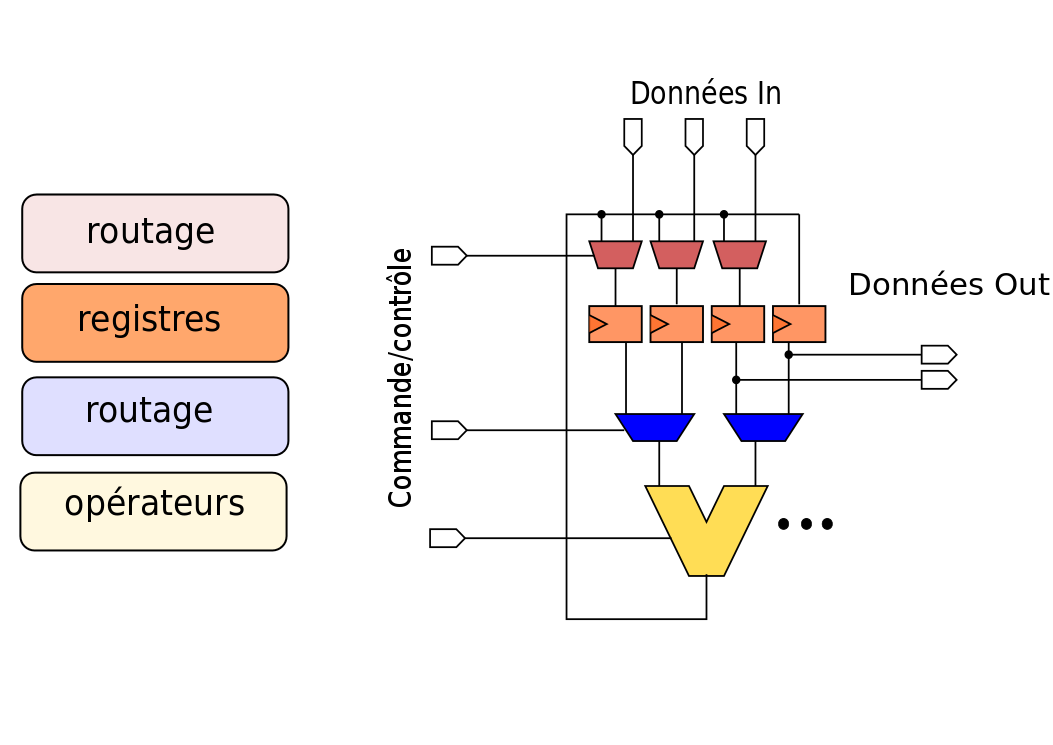
\includegraphics[width=10cm]{./figures/FSMD-1.png}
  \caption{Architecture générique d'un chemin de données. On notera les pointillés, qui indique que l'architecture peut être étendue en respectant le motif.}
  \label{fig:fsmd1}
\end{figure}

Cette architecture peut être étendue, de sorte qu'il devient possible d'effectuer plusieurs calculs en même temps : on peut réaliser un {\bf parallélisme d'instructions}.

\section{Schéma générique d'architecture contrôleur-datapath}

Le schéma \ref{fig:fsmd2} du datapath précédent ne précisait pas l'origine des commandes des multiplexeurs. D'où viennent-elles ?
Ces multiplexeurs sont commandés par des commandes émanant d'un contrôleur, qui n'est ni plus ni moins qu'un automate d'états finis (FSM).
On se retrouve donc avec un schéma plus élaboré, exposé sur la figure \ref{fig:fsmd2}. On se limite au cas simple où les automates sont de type Moore, c'est-à-dire
dont les sorties (ici les commandes) ne dépendent que de l'état courant.

\begin{itemize}
  \item Le contrôleur réalise le séquencement d'un ensemble de calculs.
  \item Dans chaque état, le contrôleur envoie différentes actions au datapath : ces actions sont les valeurs des multiplexeurs du datapath.
  \item En retour, le contrôleur peut observer certains bits de status, stockés dans des registres. Selon ces bits (généralement des résultats de comparaison),
  le contrôleur décide vers quel état il doit transiter.
\end{itemize}

\begin{figure}[h!]
  \centering
   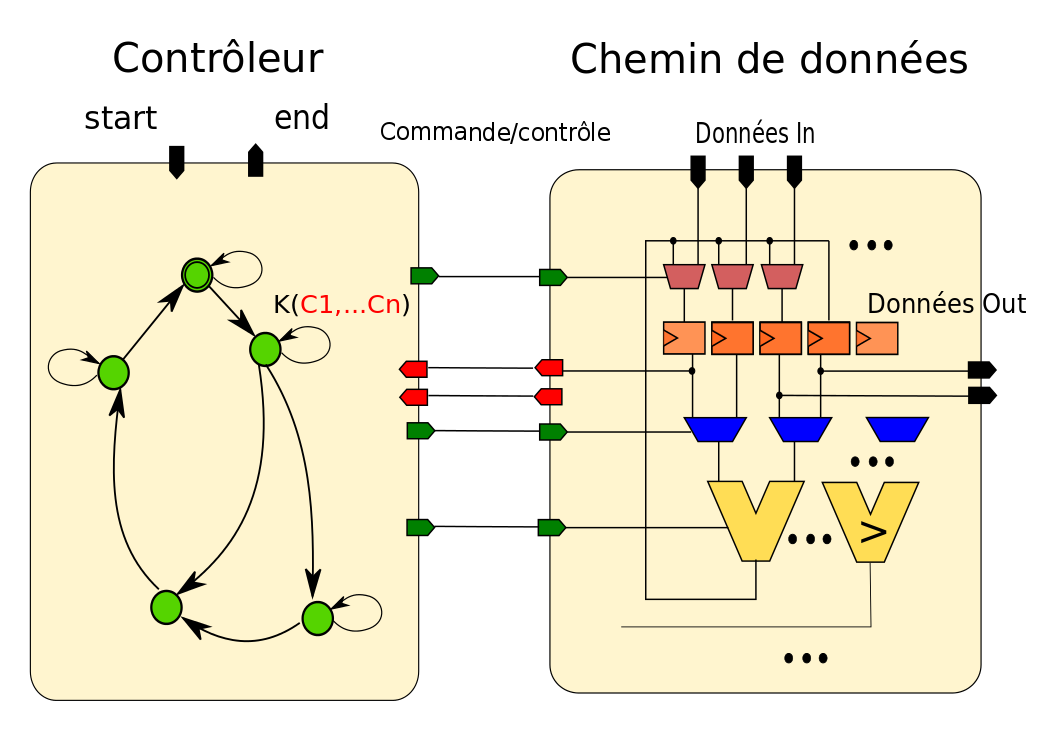
\includegraphics[width=10cm]{./figures/FSMD-2.png}
  \caption{Automates de Moore et de Mealy}
  \label{fig:fsmd2}
\end{figure}

La composition du contrôleur et du chemin de données conduit à une microarchitecture, très proche d'un coeur de microprocesseur. On la retrouve dans la littérature
anglo-saxonne sous le vocable de {\bf FSMD} : FSM + Datapath.

\section{Exercice}
A titre d'exercice, on propose l'énoncé suivant : on cherche à réaliser le calcul d'une droite $y=ax+b$ pour $x$ variant de 0 à 100.
Après appui sur un bouton "go", les deux coefficients arrivent sur le port P1, en séquence. Réaliser l'architecture FSMD de ce calculateur en faisant l'hypothèse
qu'on ne dispose que d'une unité de calcul. Ecrire un pseudo-code logiciel et un schéma détaillé de contrôleur et de chemin de données.

\section{Conclusion}
Ce court chapitre permet de comprendre un motif classique de conception de circuits numérique : le couple contrôleur-chemin de données (FSMD). L'utilité de
tous les composants, dont nous avons préalablement établi les équations logiques constitutives, commence à se faire jour. A la manière de poupées gigognes,
les systèmes numériques vont pouvoir devenir de plus en plus complexes, bien que tous basés sur des principes simples. Les étapes suivantes, que nous étudierons
plus tard, consistent à établir une stratégie pour convertir tout algorithme en architecture FSMD : c'est un accélérateur de calcul dédié.
Dans le cas où le contrôleur cablé est remplacé par un contrôleur plus flexible et reprogrammable, nosu aboutissons à un microprocesseur.
